%============================= BACKGROUND =================================

% Often used notations
\def\x{\mathbf{x}} % input vector
\def\X{\mathbf{X}} % input dataset

\def\y{\mathbf{y}} % target/output vector
\def\Y{\mathbf{Y}} % target/output dataset

\def\w{\mathbf{w}} % weight vector
\def\W{\mathbf{W}} % weight matrix
\def\b{\mathbf{b}} % bias vector

\def\z{\mathbf{z}} % aux variable (logits)
\def\h{\mathbf{h}} % hidden state
\def\o{\mathbf{o}} % output variable
\def\p{\mathbf{p}} % vector of probabilities

\def\i{\mathbf{i}} % lstm input gate
\def\f{\mathbf{f}} % lstm forget gate
\def\o{\mathbf{o}} % lstm output gate
\def\u{\mathbf{u}} % lstm update gate
\def\c{\mathbf{c}} % lstm cell state

\def\R{\mathbb{R}} % real numbers
\def\L{\mathcal{L}} % loss function
\def\a{\varphi} % activation function

\def\({\left (} % left par
\def\){\right )} % right par


\chapter{Background}
\label{ch:background}

% TODO add overfit, underfit to background?
% TODO add train good practices? (train/val/test splits, epochs, etc.)
% TODO add dropout to regularizations

In this chapter, we present the basic concepts about \gls{dl}, and we introduce the research fields on which its application has been investigated in this thesis, namely Image Classification and \gls{cbir}.
% TODO add some more intro to the bg chapter?
The chapter is organized as follows.
In \ref{sec:back:deep-learning}, we provide the reader with a quick introduction to \acrlong{dl}, focusing on deep neural networks for image and text processing and gradient-based optimization.
In \ref{sec:back:image-classification}, an introduction to image classification using \acrfullpl{cnn} is presented together with a review of successful approaches in this field.
In \ref{sec:back:image-retrieval}, we describe the main aspects of \gls{cbir} based on image representations extracted from deep neural networks, and we discuss some state-of-the-art methodologies to build effecive description of images and to efficiently index them in large-scale scenarios.
\ref{sec:back:datasets} summarizes the public datasets used in the experiments presented in this thesis.


\section{Deep Learning}
\label{sec:back:deep-learning}

\acrfull{dl} defines a subfield of Artificial Intelligence, specifically of \gls{ml}, in which a \emph{hierarchy of data representations} (or \emph{features}) is learnt from data for solving a particular task~\cite{bengio2007scaling,goodfellow2016deep}.
% TODO add representation learning?, what is and cites
%For historical reasons, \gls{dl} models are also referred to as \emph{\glspl{dnn}} due to the resemblance of layers and their organization to the way neurons are interconnected and organized in the mammalian brain~\cite{}.
% TODO add reference to similarities to mammalian brain (in addition to perceptron?)
Inspired by nature, \acrlong{dl} models are often implemented as \glspl{dnn} -- a computational model comprised by multiple layers of processing units that mimics the structure and the interconnection of neurons in the mammalian brain~\cite{rosenblatt1958perceptron}.
Recent years have witnessed a rapid rise in the use of \gls{dl} approaches to solve complex task, reaching even super-human performance in perceptiual~\cite{he2015delving}, control~\cite{mnih2015human}, and planning~\cite{silver2016mastering} activities. % TODO add reasoning?
Interestingly, the representations learnt with \gls{dl} methodologies resemble the structures of signals in the neocortex build by our brain to implement intelligent behaviours, suggesting a strong parallelism between the two~\cite{cadieu2014deep,kubilius2016deep}. % TODO dire meglio

\acrlongpl{dnn} are organized as a sequence (or more generally a graph) of parametric non-linear transformations, known as \emph{layers}, that acts like features extractors;
starting from raw data, each layer searches for useful patterns in its input and provides higher-level representation of the data to the next layer.

Formally, given an input $\x$, we can express the output $\y$ of \gls{dnn} as
%
\begin{equation} \label{eq:back:deepnet}
    \y & = f\(\x, \Theta\)
%\begin{split}
%    \y & = f\(\x, \Theta\) \\
%       & = f_L\(\dots f_2\(f_1\(\x; \theta_1\); \theta_2\); \theta_L\) \,,
%\end{split}
\end{equation}
%
where $f(\cdot)$ is an arbitrary composition of parametric transformations (layers), and $\Theta$ indicates the set of all the parameters, also known as \emph{weights} of the \gls{dnn}.

Given a training set of input-target couples $\X = \{ (\x_i, \y_i^\star),\; i = 1, \dots, N \}$, the quality of a particular setting of parameters is quantitatively defined by a \emph{loss function} $\L\(\X; \Theta\)$ that measures how much the model predictions $\y$ differ from the targets $\y^\star$ provided by $\X$.
The particular formulation of $\L$ is task-dependent and further discussed in \ref{subsec:back:loss}.
In the end, the learning problem reduces to the optimization problem
%
\begin{equation} \label{eq:back:optim}
    \Theta^\star = \argmin_\Theta \L\(\X; \Theta\) \,,
\end{equation}
%
in which we search the best parameter setting $\Theta^\star$ that minimizes the loss function $\L\(\X; \Theta\)$.

The specific layers used and their interconnections define the \gls{dnn}'s \emph{architecture} (or \emph{computation graph}).
\Glspl{dnn} can be roughly categorized into \glspl{ffnn}, in which information flows from input to output in a non-recursive cascade of computations, and \glspl{rnn}, which present a feedback loop in their computation graph.
In the following sections, we will review some practical and successful formulations of \glspl{dnn},
%that are useful when dealing with image data
and we will provide the reader with the basics of gradient-based optimization of \ref{eq:back:optim}.

\subsection{Feed-Forward Neural Networks}
\label{subsec:back:ffnn}

\Acrlongpl{ffnn} are networks whose computation graph can be expressed as a directed acyclic graph, i.e.\,there are no feedback loops and information flows from inputs to outputs in a cascade fashion.
Thus, when computing of the whole chain from inputs to outputs, called the \emph{forward} pass of the network, each transformation defined by layers is computed only once.

% In the following, we summarize some of the most relevant layers used in \glspl{dnn}.

%\subsubsection{Fully Connected Layer}
\subsubsection{Multilayer Perceptrons}

\begin{figure}
    \includegraphics[ width=\linewidth]{figures/activations}
    \caption{Commonly used activation functions in \glspl{dnn}. The \acrfull{relu} on the left, the sigmoid $\sigma$ in the middle, and hyperbolic tangent on the right.}
    \label{fig:back:activations}
\end{figure}

The \gls{mlp} is the simplest form of artificial neural network in the \Acrlong{dl} field.
A \gls{mlp} is comprised by a cascade of \emph{inner product} (or \emph{fully connected}) layers, which are the basic building block for \glspl{dnn}.
A inner product layer performs a linear projection of the input followed by a usually non-linear element-wise activation function.
Formally, given an input comprised by $n$ features $\x \in \R^n$, the output  $\y \in \R^m$ of the layer is obtained as
%
\begin{equation} \label{eq:back:fully-connected}
    \y = \a \( \W \x + \b \) \,,
\end{equation}
%
where $\W \in \R^{n \times m}$ and $\b \in \R^m$ are learnable parameters of a linear projection to a $m$-dimensional space.
Commonly used activation functions $\a: \R \to \R$ are the \gls{relu}, the sigmoid $\sigma\(\cdot\)$, or $\tanh\(\cdot\)$ functions (depicted in~\ref{fig:back:activations}).
The dimensionality of the input $n$ and of the output $m$ are referred to as respectively the number of \emph{input features} and \emph{output features}.

\begin{figure}
    \centering
    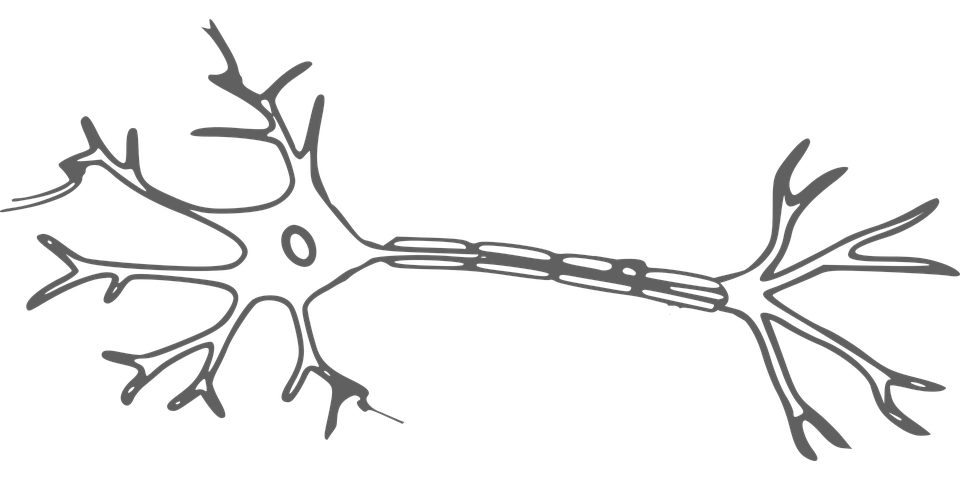
\includegraphics[width=0.8\linewidth]{figures/neuron}
    \caption{Parallelism between a real neuron and the artificial one used in \glspl{mlp}}
    \label{fig:back:neuron}
\end{figure}

Historically, this layer implemented a group of $m$ \emph{perceptrons}.
The perceptron~\cite{rosenblatt1958perceptron} is a biologically-inspired building block for artificial neural networks that has been developed mimicking the structure of biological neurons (see \ref{fig:back:neuron}).
As a neuron cell, it is composed by $n$ inputs $\x_i$ ($i=1 \dots n$), usually connected to the output of other neurons, and a single output $\mathbf{y}$ (axon).
Each input connection is associated with a weight $\w_i$ ($i=1 \dots n$) expressing how much of the signal coming through that connection is promoted or inhibited.
Weights in a perceptron are interpreted as the strength of the interconnection between neuron cells.
The neuron ``fires'' when the combination of their weighted inputs gets above a certain threshold;
this is modelled in the perceptron defining its output as the activation function $\a$ applied to the inner product between input and weights
%
\begin{equation}
    \y_j = \a \( \sum_{i=1}^n \w_i \x_i + b\) \,,
\end{equation}
%
where $\y_j$ is the output of a particular neuron and $b \in \R$ is an optional weight used as bias term.
% The weight vector $\w$ is tuned in the training phase in order to
A layer composed by $m$ perceptrons (and thus $m$ outputs $\y_j, j=1 \dots m$) sharing the same input $\x$ can be formalized with \ref{eq:back:fully-connected}, where the columns of $\W$ correspond to the weights of the $m$ perceptrons.
% Feed-forward artificial neural networks built stacking layers of perceptrons are called \glspl{mlp}.
In \glspl{mlp}, the outputs of a layer are densely connected to the input of each neuron comprising the next layer, hence the name ``fully-connected layer''.
The output of a \gls{mlp} with $L$ layers is defined as
%
\begin{equation}
    \y = \a \( \W_L \( \dots \a \( \W_2 \( \a \( \W_1 \x + \b_1 \) \) + \b_2 \) \) + \b_L \) \,,
\end{equation}
%
where $\(\W_i, \b_i \)$ are the parameters of the $i$-th fully-connected layer in the network.

\subsubsection{Convolutional Neural Networks}

\begin{figure}
    % TODO add subfigure with example of crosscorr on image
    \centering
    \includegraphics[width=0.5\linewidth]{figures/cross-correlation2d}
    \caption{Example of cross-correlation between 2D signals}
    \label{fig:back:2d-cross-corr}
\end{figure}

A \gls{cnn} is a feed-forward artificial neural network composed by at least one \emph{convolutional} layer.
This kind of layer computes the cross-correlation between the input and a set of learnable filters.
Since there is a strong similarity between the convolution and the cross-correlation operations, this layer is often attributed with the adjective ``convolutional'' in the \gls{dl} literature;
thus we will adopt the same terminology throughout this thesis.

\paragraph{Cross-correlation}
The \emph{cross-correlation} (also called \emph{sliding inner product}) is typically used in signal processing to search for matches between two signals.
Intuitively, a small signal called \emph{filter} containing the prototype we want to match is slided on a bigger input signal, and for each position, the inner product between the intersection of the two signals measures the quality of the match.
We will provide the reader with the formulation of the two-dimensional version of the cross-correlation due to its massive adoption in image-related fields that are of interest for this work.

Given a two-dimensional input matrix $\x \in \R^{H \times W}$ and a two-dimensional filter $\w \in \R^{K_1 \times K_2}$, %with $K \ll \min(H,W)$,
the cross-correlation $\y \in \R^{H' \times W'}$ between $\x$ and $\w$ is given by
%
\begin{equation}\label{eq:back:cross-correlation}
    \y_{u,v} = \sum_{i=1}^{K_1} \sum_{j=1}^{K_2} \w_{i,j} \x_{i+u-1,j+v-1} \,,
\end{equation}
%
where $u = 1, \dots, H'$ and $v = 1, \dots W'$.
Intuitively, the filter $\w$ is superimposed on the input $\x$, and for each possible position $(u,v)$, the scalar product between the covered input and the filter is computed.
Depending on the presence of padding $P$ added to each side of the input and the stride $S$ of the filter application, the output dimensionality changes following the relations
\begin{equation} \label{eq:back:conv-size}
\begin{split}
    H' = \left \lfloor \frac{H + 2 \times P - K_1}{S} \right \rfloor + 1 \,,\quad
    W' &= \left \lfloor \frac{W + 2 \times P - K_2}{S} \right \rfloor + 1 \,.
\end{split}
\end{equation}
Inputs and outputs of convolutional layers are also called \emph{feature maps}, since high values in the two-dimensional map is usually interpreted as the presence of a feature a particular filter has learnt to identify.
A depiction of 2D cross-correlation is reported in~\ref{fig:back:2d-cross-corr}.

\begin{figure}
    \centering
    \includegraphics[width=\linewidth]{figures/convolution}
    \caption{Depiction of 2D cross-correlation on volumes implemented in convolutional layers}
    \label{fig:back:convolution}
\end{figure}

\paragraph{2D Cross-correlation on Volumes}
\ref{eq:back:cross-correlation} defines the cross-correlation operation for inputs and outputs having both a single feature map.
Images instead are represented as 3-D tensors having $C$ channels (e.g. $C=3$ for RGB data, $C=1$ for grayscale) and two spatial dimensions $H$ and $W$;
thus, the definition of the 2D cross-correlation is extended to 3D tensors letting the filters span the depth of the input tensor.
In such way, filters are still applied over the two spatial dimensions $H$ and $W$, but each output value depends on all the input feature maps in a particular spatial position.
Formally, given an input tensor $\x \in \R^{H \times W \times C}$ and a filter $\w \in \R^{K_1 \times K_2 \times C}$ the cross-correlation $\y \in \R^{H' \times W'}$ between $\x$ and $\w$ is defined as
%
\begin{equation}\label{eq:back:channel-cross-correlation}
    \y_{u,v} = \sum_{i=1}^{K_1} \sum_{j=1}^{K_2} \sum_{k=1}^C \w_{i,j,k} \x_{i+u-1,j+v-1,k} \,.
\end{equation}

A convolution layer is often composed by a bank of $K$ filters.
Each filter is applied to the input, obtaining $K$ output feature maps that are stacked along the depth dimension.
The obtained output is a new 3D tensor $\y \in \R^{H' \times W' \times K}$ that is commonly followed by an element-wise non-linear activation $\a$.
The entire process is depicted in \ref{fig:back:convolution}.

The main difference between fully-connected layers and convolutional layers is the way weights are utilized;
while fully-connected layers have a dedicated weight for each couple of input and output features, a convolutional layer shares the weights of its filters across the spatial dimensions, thus learning to detect translation-invariant features by design.

\paragraph{Pooling Layers}
Pooling layers are often used in \glspl{cnn} to reduce the amount of data to be processed in the next layers.
As the name suggests, this kind of layers pools data in groups and aggregates them using a non-parametric aggregation function, such as maximum or average.
The groups are defined as fixed-size windows that are slided along one or more dimensions of the data in the same way the cross-correlation operator is applied.
In the two dimensional case, input and output sizes follow \ref{eq:back:conv-size}.
The application of convolutional layers having small strides usually produce redundant local information in their output.
Thus, a max-pooling layer is often used to reduce the resolution of intermediate feature maps.
% Instead, sum- and average-pooling are used to produce

\paragraph{Features hierarchy in \glspl{cnn}}
% TODO add some cites of successful CNNs in DL literature
Convolutional layers are stacked to build deep \glspl{cnn}, that are the one of the core tools of Deep Learning for image perception and analysis \cite{}.
Once trained, filters in a deep \gls{cnn} tend to organize in a hierarchy of detectors, where layers near the input detect the presence of simple features in the input data, while the following layers build up from them and detect more complex features.
A successful example of the representative power of \glspl{cnn} is object recognition.
% TODO add a cite to object decomposition
The visual aspect of object is images follow a hierarchical organization: an object can be decomposed in parts, parts in patches, patches in textures, texture in edges or blobs, and finally in pixels \cite{}.
\begin{figure}
    % TODO is feat hier figure valuable?
    \centering
    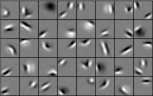
\includegraphics[height=2.9cm]{img/feat-hier-1.png}%
    \hfill%
    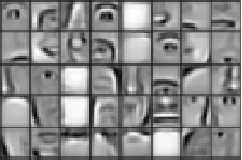
\includegraphics[height=2.9cm]{img/feat-hier-2.png}%
    \hfill%
    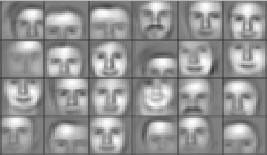
\includegraphics[height=2.9cm]{img/feat-hier-3.png}%
    \newline
    \caption{
    Visualization of the feature hierarchy learned by convolutional layers in a \gls{dl}-model trained on faces.
    Low-level features (edges and blobs, on the left) are detected and then combined to recognize parts (eyes, nose, mouth, in the middle) and finally faces (on the right).
    \figfrom{lee2011unsupervised}
    }
    \label{fig:back:filter-hier}
\end{figure}
\Glspl{cnn} trained to recognize objects, directly or indirectly, often organize their hierarchy of detectors following this kind of visual decomposition of objects (see \ref{fig:back:filter-hier}).


\subsection{Recurrent Neural Networks}
\label{subsec:back:rnn}

% TODO add rnn cites: non c'è un paper di riferimento
A \acrfull{rnn} is a stateful artificial neural network with feedback connections in which the output depends not only on the input, but also on the current state of the network~\cite{}.
The state of the network acts as a memory which is updated at each input, allowing information to persist between inputs.
This architecture is naturally able to process sequences of inputs -- elements of the sequence can be fed to the network one by one, updating the internal state of the network to compactly represent the sequence processed so far regardless of its length.
% This is achieved by adding a cycle in the computation graph --

\begin{figure}
    \centering
    \includegraphics[width=.9\linewidth]{figures/rnn}
    \caption{Basic architecture of a \acrlong{rnn} (left). On the right, its unrolled version for a sequence of length 5.}
    \label{fig:back:rnn}
\end{figure}

Given a sequence of inputs of length $T$ $\x_t \in \R^n, t = 1 \dots T$, and an initial state $\h_0 \in \R^m$, a \gls{rnn} can be described as a parametric function mapping the input and the state at a certain timestep to the next hidden state
%
\begin{equation}\label{eq:back:rnn}
    \h_t = f\(\x_t, \h_{t-1}; \W\) \,,
\end{equation}
%
where $f(\cdot)$ is the \emph{recurrent cell} of the \gls{rnn} parametrized by the weights $\W$, and $\h_t \in \R^m, t = 1 \dots T$ is the hidden state at timestep $t$, i.e.\ the state of the network after all inputs until $\x_t$ have been processed.
In its simplest form, the recurrent cell $f$ can be implemented using a fully-connected layer that operates
on the concatenation of the current state and input
%
\begin{equation}
    \h_t = \W [ \x_t | \h_{t-1} ] + \b \,,
\end{equation}
%
where $\W$ and $\b$ are the parameters of a fully-connected layer, and $[\cdot|\cdot]$ is the concatenation operation.
During learning, the \gls{rnn} is unrolled in time to the length of the input sequence to create an acyclic computation graph similar to \glspl{ffnn} (see \ref{fig:back:rnn}) on which standard training procedures can be applied (that will be discussed in \ref{subsec:back:optim}).
Depending on the task we want to model, we could be interested in the last hidden state $\h_T$ compactly represent the whole sequence, or we could use a combination of all hidden states $\h_i, i=1 \dots T$ to get access to the evolution of the information processed through time.

\paragraph{Bidirectional \glspl{rnn}}
In many tasks such as sequence classification and segmentation, also the future context of the sequence is informative. However, \ref{eq:back:rnn} defines a \gls{rnn} encoding only past information, i.e.\   $\h_t$ depends only on information at time step $t' < t$.
To overcome this limitation, \emph{bidirectional} \glspl{rnn} have been proposed~\cite{schuster1997bidirectional}.
Bidirectional architectures adds a separate recurrent cell which process the sequence in reverse order (from future to past)
%
\begin{equation}
    \h'_t = f'\(\x_t, \h'_{t+1}; \W'\) \,,
\end{equation}
%
where $\h'_t$ encodes the "future" part of the sequence, i.e.\ depends on information at time step $t' > t$.
The concatenation of the internal states of both past-to-future and future-to-past \glspl{rnn} $[\h_t | \h'_t]$ is often used as the representation of the whole sequence.

\begin{figure}
    \centering
    \includegraphics[width=.9\linewidth]{figures/bidir-rnn}
    \caption{Unrolled version of a Bidirectional \gls{rnn} for a sequence of length 5}
    \label{fig:back:bidir-rnn}
\end{figure}

\subsubsection{Long Short-Term Memory}

% TODO add LSTM application cites
\Gls{lstm}~\cite{hochreiter1997long} is a type of \gls{rnn} with a special formulation of the recurrent cell that has proved its effectiveness in several sequence-modeling tasks~\cite{}.
This particular formulation is aimed at solving some major drawbacks of vanilla \glspl{rnn}, most importantly the inability to encode long-term dependencies in long sequences due to gradient instability problems, namely the problem of vanishing or exploding gradients ~\cite{pascanu2013difficulty}.
\Gls{lstm} cells are comprised by four learnable gating functions that better control the evolution of the internal state of the cell when dealing with long sequences, and mitigating problems occurring in vanilla RNNs, such as vanishing gradients~\cite{bayer2015learning}.

Let $\x_t \in \R^n$ an element of a sequence, and $\h_{t-1} \in \R^m$ the current hidden state.
The \emph{forget} gate $\f_t$ decides which information need to be discarded at the current step, and it is implemented as a fully-connected layer with $p$ output features and parameters $\w_f \in \R^{(n+m)\times p}, \b_f \in \R^p$ followed by a sigmoid activation
\begin{equation*}
    \f_t = \sigma\(\w_f [\h_{t-1} | \x_t] + \b_f\) \,.
\end{equation*}
The input gate $\i_t$ encodes the information that need to be inserted in the internal state of the cell $\c_t$, and it is implemented following the same rationale of the previous gate
\begin{equation*}
    \i_t = \sigma\(\w_i [\h_{t-1} | \x_t] + \b_i\) \,.
\end{equation*}
The update gate $\u_t$ modulates the amount of new input to be inserted in the internal state of the cell $\c_t$
\begin{equation*}
    \u_t = \tanh\(\w_u [\h_{t-1} | \x_t] + \b_u\) \,.
\end{equation*}
The new cell state $\c_t \in \R^p$ is computed as the sum of two terms;
the first one, given by the element-wise product ($*$) between the forget gate and the previous cell state, represents the part of the old state not to be forgotten;
the second one, computed as the element-wise product of the input and update gates, represent the modulated input to be kept in the new state;
\begin{equation*}
    \c_t = \f_t * \c_{t-1} + \i_t * \u_t \,.
\end{equation*}
The output gate $\o_t$ decides which information in the cell needs to be transferred to the final state $\h_t$
\begin{equation*}
    \o_t = \sigma\(\w_o [\h_{t-1} | \x_t] + \b_o\) \,,
\end{equation*}
and finally, the output state $\h_t$ is computed as
\begin{equation*}
    \h_t = \o_t * \tanh\(\c_t\) \,.
\end{equation*}
%
With an abuse of notation, the complete \gls{lstm} formulation can be compactly written as follows:

%\begin{align}\label{eq:back:lstm}
    % \begin{pmatrix} \i_t\\ \f_t \\ \o_t \\ \u_t \end{pmatrix}
%    \i_t &= \sigma\(\W_i [\h_{t-1} | \x_t] + \b_i\) \\
%    \f_t &= \sigma\(\W_f [\h_{t-1} | \x_t] + \b_f\) \\
%    \o_t &= \sigma\(\W_o [\h_{t-1} | \x_t] + \b_o\) \\
%    \u_t &= \tanh\(\W_u [\h_{t-1} | \x_t] + \b_u\) \\[2ex]
%    \c_t &= \f_t * \c_{t-1} + \i_t * \u_t \\
%    \h_t &= \o_t * \tanh\(\c_t\)
%\end{align}
\begin{align}\label{eq:back:lstm}
\begin{aligned}
    \begin{pmatrix} \i_t\\ \f_t \\ \o_t \\ \u_t \end{pmatrix} &=
    \begin{pmatrix} \sigma \\ \sigma \\ \sigma \\ \tanh \end{pmatrix}
    \( \W \begin{pmatrix} \x_t \\ \h_{t-1} \end{pmatrix} \) \\[2ex]
    \c_t &= \f_t * \c_{t-1} + \i_t * \u_t \\
    \h_t &= \o_t * \tanh\(\c_t\) \,,
\end{aligned}
\end{align}
%
where $\W \in \R^{(n+m) \times 4p}$ summarizes all the parameters of all the fully-connected layers forming the gates.
% TODO: [PLUS] lstm figure
A depiction of the \gls{lstm} cell is aslo available in \ref{fig:back:lstm}.

\begin{figure}
    \centering
    \includegraphics[width=\linewidth]{figures/lstm}
    \caption{Example of \gls{lstm} cell}
    \label{fig:back:lstm}
\end{figure}

\subsection{Loss Functions}
\label{subsec:back:loss}

Loss functions are a key component of \gls{ml} methods.
Its role is to quantitatively assign a value of goodness to a model in reference to the particular task we want to solve.

Given a training set $\X = \{\(\x_i, \y^\star_i\),\; i=1,\dots,N\}$ comprised by $N$ couples of inputs and desired outputs, the quality of a particular setting of parameters $\Theta$ is quantitatively defined by a \emph{loss function} $\L\(\X; \Theta\)$ that measures how much predictions and targets differ.
A loss function is usually defined as one of more terms summed together.
The main term $\L_d\(\X; \Theta\)$ is defined as the average of the individual loss values computed on each sample of the dataset $\L\(\y_i, \y^\star_i\)$ -- we denote it the \emph{data term}.
A secondary optional term $\L_r(\Theta)$ is often used to regularize the network and depends only on the model parameters $\Theta$ -- we indicate this as \emph{regularization term}.
Regularization consists of model constraints added to avoid other undesired properties during training.
Regularization has gained importance in the \gls{dl} field due to the huge amount of parameters models are usually comprised of, thus increasing the risk of \emph{overfit} on the train data.
The regularization term is usually multiplied by a hyperparameter $\alpha$ and then added to the loss function.
A general formulation of the loss function is
%
\begin{equation} \label{eq:back:loss}
\begin{aligned}
    \L\(\X; \Theta\) &= \overbrace{\L_d\(\X; \Theta\)}^{\textrm{data term}}&+\, \alpha &\overbrace{\L_r\(\Theta\)}^{\textrm{regularization term}}\\
                     &= \frac{1}{N} \sum_{i=1}^N \L\(\y_i, \y^\star_i\)&+\alpha & \,\quad \L_r\(\Theta\) \\
                     &= \frac{1}{N} \sum_{i=1}^N \L\(f\(\x_i; \Theta\), \y^\star_i\)&+\alpha & \,\quad\L_r\(\Theta\) \,.
\end{aligned}
\end{equation}
%
%where the optimal value of $\alpha depends on the absolute values of the loss terms and

In the next paragraphs, we will provide the reader with some of the most used formulations of $\L\(\y_i, \y^\star_i\)$ and $\L_r(\Theta)$ of interest for this work.

\paragraph{Mean Squared Error Loss}
When dealing with regression problems, we want our predictions to be close to the one or more real-valued targets.
For example, in an age estimation problem, we want our network to predict the exact age expressed as a real value, e.g. $46,5$.
The mean squared error between predictions $\z$ and targets $\z^\star$ is a commonly used loss function to measure the goodness of regressions
\begin{equation} \label{eq:back:mse}
    \L_\textrm{MSE}(\z, \z^\star) = \frac{1}{2} \( \z - \z^\star \)^2 \,.
\end{equation}
%
The scale factor $\frac{1}{2}$ is usually introduced to simplify the gradient computation when using this loss function (more details on this in \ref{subsec:back:optim}).

\paragraph{Cross-entropy Loss}
The cross-entropy loss is commonly used in \gls{ml} to measure the distance between two categorical distributions.
It is commonly adopted in single-label classification tasks, where a single label have to be assigned to a piece of data choosing from $N$ labels ($N \geq 2$).
Let $\z$ and $\z^\star$ the probability masses of two $N$-way categorical distributions, i.e. $\z_i, \z^\star_i \in [0,1],\; \sum_{i=1}^N \z_i = 1, \sum_{i=1}^N \z^\star_i = 1$;
the cross-entropy loss between the predicted distribution $\z$ and the target one $\z^\star$ is defined as
%
\begin{equation} \label{eq:back:cross-entropy}
    \L_\textrm{CE}(\z, \z^\star) = - \sum_{i=1}^N \z^\star_i \log \z_i \,.
\end{equation}
%
Classification models are often designed to output a $N$-dimensional vector $\z$ that is mapped to a categorical distribution via the \emph{softmax} function
%
\begin{equation} \label{eq:back:softmax}
    \textrm{softmax}(\z)_i = \frac{e^{\z_i}}{\sum_{j=1}^N e^{\z_j}} \,.
\end{equation}

\paragraph{$\mathbf{L_p}$ weight decay}
The most used regulatization terms in the \gls{dl} literature are the ones penalizing the parameters having large norm.
This is usually implemented defining the regularization term $\L_r\(\Theta\)$ added to the loss to be minimized as the $p$-norm of the parameters.
Practical definitions have been adopted for $p=2$ ($\mathbf{L_2}$ weight decay) and for $p=1$ ($\mathbf{L_1}$ weight decay).
The former produces a more uniform utilization of all the available parameters, penalizing under-utilized and over-utilized weights~\cite{ng2004feature}, and is defined as
%
\begin{equation} \label{eq:back:l2-weight-decay}
    \L_r\(\Theta\) = \frac{1}{2} ||\Theta||_2^2 = \frac{1}{2} \sum_i \theta_i^2 \,.
\end{equation}
%
The latter instead tends to produce a more sparse weight configuration, i.e. with many parameters having a null optimal value~\cite{ng2004feature}, and is defined as
%
\begin{equation} \label{eq:back:l1-weight-decay}
    \L_r\(\Theta\) = ||\Theta||_1 = \sum_i |\theta_i| \,.
\end{equation}

\subsection{Gradient-Based Optimization}
\label{subsec:back:optim}

As already stated, solutions of \ref{eq:back:optim} are the parameter configurations $\Theta$ that minimizes the loss function $\L$ defined over a given training set $\X$.
% TODO add something abound convexness of loss, citing bengio2007scaling
Unfortunately, in very rare cases closed-form solutions of \ref{eq:back:optim} are available for practical formulations of \gls{dl} models $f(\cdot)$.
Instead, suboptimal solutions can be found using iterative gradient-based optimization.

\paragraph{Gradient Descent}
In gradient-based optimization, given a training set $\X$ and a parameter configuration $\Theta$, we search for a new solution following the direction of the gradient of the loss function $\nabla\L\(\X, \Theta\)$ with respect to the parameters $\Theta$.
The direction given by $\nabla\L\(\X, \Theta\)$ is the one of maximum steepness of the loss surface in the parameter space, that is, the one that maximize the loss change locally.
A new parameter configuration $\Theta^\star$ is chosen \emph{descending} the loss surface along the direction of maximum steepness with a step size of $\lambda$, that is
%
\begin{equation} \label{eq:back:gradient-descent}
    \Theta^\star = \Theta - \lambda \nabla\L\(\X, \Theta\) \,.
\end{equation}
%
This update rule can be iterated until a (local or global) minimum of the loss function is reached.
This procedure is called \emph{gradient descent} optimization, and in the \gls{ml} field $\lambda$ is referred to as the \emph{learning rate}.
\begin{figure}
    \centering
    \includegraphics[width=\linewidth]{figures/gradient-descent}
    \caption{Example of gradient descent optimization on a loss surface $\L(\X)$ defined over a 2D parameter space $(\w_1, \w_2)$ with two different starting points}
    \label{fig:back:gradient-descent}
\end{figure}
A depiction of this algorithm for a 2D toy example is reported in \ref{fig:back:gradient-descent}.
Bigger learning rates correspond to bigger steps along the loss surface that usually improve the convergence rate and avoid local minima at the cost of a higher risk of oscillating around minimum points.
Small learning rates, instead, bring a lower convergence rate but are able to better exploit the local topology of the loss function, reaching a locally better solution.

\paragraph{Back-propagation}
As formalized in \ref{eq:back:deepnet}, \glspl{dnn} are comprised by many composition of non-linear functions $f_i$ each having its own set of parameters $\theta_i$.
Thus, to perform gradient descent on \gls{dl} models, we need to compute gradients $\nabla\L\(\X, \theta_i\)$ for each $\theta_i \in \Theta$.
This is efficiently done by \emph{back-propagation}~\cite{rumelhart1986learning,lecun1988theoretical}.

In back-propagation, we start computing the gradient of the loss function from the last layer (the one that produce the final predictions), and we propagate the error backwards to previous layers using the chain-rule for computing derivatives of compound functions.
For simplicity, we report the formulation of back-propagation for a \acrfull{ffnn}, but this mechanism is general and applies to all differentiable architectures.
Let $f(\x;\Theta)$ a \gls{ffnn} composed by $L$ layers with parameters $\Theta = \{\theta_1, \dots, \theta_L\}$ defined in \ref{eq:back:deepnet}, and let $\o_i$ the output of the $i$-th layer
\begin{equation}
\begin{split}
\o_0 &= \x \\
\o_i &= f_i \(\o_{i-1}; \theta_i \) \,.
\end{split}
\end{equation}
The gradient $\frac{\partial \L}{\partial \theta_i}$ of the loss function $\L$ with respect to $\theta_i$ can be decomposed using the chain-rule as
\begin{equation}
\begin{split}
    \frac{\partial \L}{\partial \theta_i} &= \frac{\partial \L}{\partial \o_i} \cdot \frac{\partial \o_i}{\partial \theta_i} \\
                                          &= \frac{\partial \L}{\partial \o_L} \cdot \frac{\partial \o_L}{\partial \o_{L-1}} \cdots  \frac{\partial \o_{i+1}}{\partial \o_i} \cdot \frac{\partial \o_i}{\partial \theta_i} \,,
\end{split}
\end{equation}
%
where the partial derivatives $\frac{\partial \o_{i+1}}{\partial \o_i}$ and $\frac{\partial \o_i}{\partial \theta_i}$ are well defined and depend on the implementation of the $i$-th layer $f_i$.
The formulations of the loss function $\L$ and intermediate layers $f_i$ are chosen to be differentiable to ensure that also the entire model -- being a composition of differentiable functions -- is in turn differentiable, and that back-propagation can be applied to efficiently compute gradients.


\paragraph{Stochastic Gradient Descent}
In our presentation of gradient-based optimization so far, the computation of the loss function $\L\(\X; \Theta\)$ and its gradient depend on the whole dataset $\X$.
This may be limiting for \gls{dl} applications where very large training sets are needed to train models, thus increasing the computational cost needed to compute the exact value of $\L\(\X; \Theta\)$.
To overcome this problem, \gls{sgd} and in particular mini-batch \gls{sgd}~\cite{rumelhart1986learning} have been proposed to compute an estimate the loss function and its gradients at a lower computational cost.

In mini-batch \gls{sgd}, we use a small random sample of the entire training set $ \tilde{\X} = \{ (\tilde{\x_i}, \tilde{\y_i}), i = 1 \dots B \} \subset \X$ (called \emph{batch} or \emph{mini-batch}) to compute an estimate of loss function
\begin{equation} \label{eq:back:minibatch-sgd}
\tilde{\L} \(\X; \Theta\) = \L (\tilde{\X}; \Theta) = \frac{1}{B} \sum_{i=1}^B \L(f(\tilde{\x_i}; \Theta), \tilde{\y_i}) \,,
\end{equation}
which in turn is used in back-propagation to estimate its gradient $\nabla \L(\tilde{\X}; \Theta)$ and perform the parameter update as specified in \ref{eq:back:gradient-descent}.
The size of the mini-batch size $B$ is a hyperparameter that controls the trade-off between the computational cost needed to compute the loss and the quality of the loss estimate.

\paragraph{\gls{sgd} with Momentum}
A successful proposal to improve the parameter update rule presented in \ref{eq:back:gradient-descent} is \gls{sgd} with \emph{momentum}~\cite{qian1999momentum}.
The key idea of momentum is to add to the current direction given by the loss gradient a fraction of the direction computed in the previous iteration, such that the direction we are following to descend the loss surface gains inertia and smooths out eventual oscillations given by very steep loss manifolds.
Given $m^{(k-1)}$ the direction of the previous iteration, we define the new direction to follow $m^{(k)}$ as
\begin{equation} \label{eq:back:momentum}
\begin{aligned}
    m^{(0)} &= 0 \\
    m^{(k)} &= \gamma m^{(k-1)} + \nabla\L\(\X; \Theta^{(k)}\) \\
    \Theta^{(k+1)} &= \Theta^{(k)} - \lambda m^{(k)} \,,
\end{aligned}
\end{equation}
%
where $\gamma \in (0,1)$ is the momentum of the previous direction.
Commonly used values for $\gamma$ are around $0.9$.
A good analogy to comprehend the rationale behind momentum is a ball pushed down a hill:
the higher the momentum $\gamma$, the more inertia the ball has, and the less it is influenced by steepness variations during the descent.
This modified update rule tends to discard the oscillating directions of the gradient while strengthening the stable directions over iterations;
this brings a reduction of oscillations while descending the loss manifold and thus a faster convergence.

\paragraph{Adam}
Another widely used parameter update rule in the \gls{dl} literature is \gls{adam}~\cite{kingma2014adam}.
Similar to other proposed update rules (such as Adagrad~\cite{duchi2011adaptive} or Adadelta~\cite{zeiler2012adadelta}), this method computes an adaptive learning rate for each parameter to be optimized based on the second moment of the gradients (i.e. squared gradients), but in addition, it also estimates the first moment (the mean of the gradient itself) as in \gls{sgd} with momentum
%
\begin{equation} \label{eq:back:adam-moments}
\begin{aligned}
    m^{(k)} &= \beta_1  m^{(k-1)} + \(1 - \beta_1 \)  \nabla\L\(\X; \Theta^{(k)}\) \\
    v^{(k)} &= \beta_2  v^{(k-1)} + \(1 - \beta_2 \)  \nabla\L\(\X; \Theta^{(k)}\)^2 \,.
\end{aligned}
\end{equation}
%
The hyperparameters $\beta_1$ and $\beta_2$ are respectively controlling the aggressiveness of the exponential average of the two moments $m^{(k)}$ and $v^{(k)}$.
Since the initial values of the moments are initialized to zero, the authors propose to use the bias-corrected version of the moments, that is
%
\begin{equation} \label{eq:back:adam-moments-bias}
\begin{aligned}
    \hat{m}^{(k)} &= \frac{m^{(k)}}{1 - \beta_1^k} \\
    \hat{v}^{(k)} &= \frac{v^{(k)}}{1 - \beta_2^k} \,.
\end{aligned}
\end{equation}
%
Finally, moments estimates are used to formulate the \gls{adam} update rule
%
\begin{equation} \label{eq:back:adam}
\theta^{(k+1)}_i &= \theta^{(k)}_i - \frac{\lambda}{\sqrt{\hat{v}^{(k)}_i} + \epsilon} m^{(k)}_i \qquad \forall \theta_i \in \Theta \,,
\end{equation}
%
where $m^{(k)}_i$ and $\hat{v}^{(k)}_i$ are the first and second moments estimates of the gradients corresponding to parameter $\theta_i$, and $\epsilon$ is a small values to prevent division by zero.
Commonly used values for hyperparameters are $\beta_1 = 0.9$, $\beta_2 = 0.999$, and $\epsilon = 10^{-8}$, as suggested by the authors.

\section{Image Classification}
\label{sec:back:image-classification}

% TODO intro to img classification, examples and applications
% Examples (simple classif., sentiment analysis, etc.)
% Classifying images is super cool bla bla
In this section, we formally define the problem of image classification, and we analyze and review recent solutions based on \acrlong{dl}, and in particular Deep \acrlongpl{cnn}, proposed in the literature.

% TODO sentence dropped here at random
In the case of image classification, the data on which classifiers must rely on is raw pixel data, usually organized in a tensor with shape $(H, W, C)$, respectively representing the height, the width, and the number of channels of the image.

Many real-world problems in image understanding, such as object and face recognition, anomaly detection, and ..., can be formalized as classification problems.
For this reason, classification methods for images have received an increasing attention in the last decade.

\subsection{Problem Setting}
\label{subsec:back:classification}
Image classification consists of assigning one or more labels to an image $\x$ choosing from a finite set of $L$ labels.
We refer to \emph{single-label} $L$-way classification if only one label have to be picked among the $L$ available, referring to the special case in which $L=2$ as \emph{binary} classification.
If multiple labels can be assigned to a piece of data, we talk about \emph{multi-label} classification.
A multi-label $L$-way classification problem is often decomposed in $L$ independent binary classification sub-problems, each of them focusing on predicting the presence or the absence of one of the available $L$ labels.

Let $I$ the image space;
given an image to be classified $\x \in I$, a single-label $L$-way classifier is a function $f$ mapping $\x$ into the label space.
% Solving a classification problem reduces to find a suitable classifier $f$ that agrees with observed data labels.
The commonly used form of classification is \emph{probabilistic}, in the sense that soft assignments to the available labels are considered instead of hard ones.
In this case, an image $\x$ is mapped into its probability $p_i = p(\y = i | \x)$ of belonging to category $i$, for each category $i \in \{1, \dots, L\}$.
Thus, the classifier is a function $f: I \to \p$ which maps an image to the parameters $\p = (p_1, \ldots, p_L), \sum_{i=1}^L p_i = 1$ of a categorical distribution defined over the label space.
Soft assignments present a broad range of advantages with respect to hard assignments, the most important one being differentiability, which enables and facilitates gradient-based learning of models for $f$.

...
%Evaluation Metrics
\subsection{Evaluation}
\label{subsec:back:classif-eval}

In this section, we will report the most commonly used evaluation metrics to measure the quality of classification models.
Assume $\Y = (y_1, \ldots, y_n)$ is a set of predictions and $\tilde{\Y} = (\tilde{y}_1, \ldots, \tilde{y}_n)$ the set of the ground-truth labels for a single-label $L$-way classification problem, with $y_i, \tilde{y}_i \in \{1, \ldots, L\}$. % for $i \in \{1, \ldots, N\}$.

\paragraph{Confusion Matrix}
One of the fundamental tools for evaluating a set of label assignments is the \emph{confusion matrix}, which compactly reports the co-occurence of predicted and ground-truth labels.
The element $c_{ij}$ of the matrix indicates the number of times the model predicted the class $i$ for a sample belonging to class $j$.
We report in \ref{tab:back:confusion} the confusion matrix for the binary case ($L=2$) together with the terminology used to refer to particular values in the matrix.
For the binary case, many useful metrics can be computed from the confusion matrix, and we will introduce some of them in the next paragraphs.
Notice that the same metrics can be applied to cases with $L > 2$ by reformulating them as binary problems, where the one class is the positive class, and the other $L-1$ are condensed in the negative class;
metrics can be computed multiple times considering each class as the positive one and then aggregated to obtain a global metric for the classification.

\begin{table}
\newcolumntype{M}[1]{>{\centering\arraybackslash}m{#1}}
\renewcommand{\arraystretch}{1.5}

\begin{tabularx}{\linewidth}{cr|M{1.3cm}|M{1.3cm}|>{\hskip 2cm}r@{\hskip 3pt}X}
\multicolumn{4}{c}{}                                                                                                                                      & $TP=$ & True Positives, i.e. correct hits       \\
\multicolumn{2}{c}{}                                                  & \multicolumn{2}{c}{\bfseries Actual class}                                                  & $TN=$ & True Negatives, i.e. correct rejections \\
\multicolumn{2}{c}{}                                                  & \multicolumn{1}{c}{\it \small Positive} & \multicolumn{1}{c}{\it \small Negative} & $FP=$ & False Positives, i.e. false alarms      \\ \cline{3-4}
\parbox[t]{2mm}{\multirow{2}{*}{\rotatebox[origin=c]{90}{\bfseries Predicted}}} & {\it \small Positive} & $TP$            & $FP$                                    & $FN=$ & False Negatives, i.e. misses            \\ \cline{3-4}
                                                                      & {\it \small Negative} & $FN$            & $TN$                                    &  $P=$ & $TP+FN=$ Positive samples               \\ \cline{3-4}
\multicolumn{4}{c}{}                                                                                                                                      &  $N=$ & $TN+FP=$ Negative samples               \\
\end{tabularx}

\caption{Confusion matrix for a binary classification problem and the related terminology}
\label{tab:back:confusion}
\end{table}

% Accuracy
\paragraph{Accuracy} The accuracy of a classification is defined for the binary case as
\begin{equation} \label{eq:back:accuracy-binary}
    \texrm{Acc.} = \frac{TP + TN}{P + N} = \frac{TP + TN}{TP + FN + TN + FP} \,,
\end{equation}
that is the fraction of correctly classified samples.
For the general case with more than two classes, the accuracy is given by the sum of the elements on the diagonal of the confusion matrix -- which contains the counts for correct predictions -- and the total number of classified samples
\begin{equation} \label{eq:back:accuracy}
    \texrm{Acc.} = \frac{\sum_{i=1}^L c_{ii}}{|Y|} \,.
\end{equation}

% Top-K Accuracy
\paragraph{Top-$K$ Accuracy}
A common variant often used for probabilistic classifiers when many classes are considered, is the \emph{Top-$K$ Accuracy}.
Given the $L$ probabilities (or scores) assigned to a sample by the classifier, we consider the prediction correct if the ground-truth class appears in the first $K$ highest scored classes.
The metric then is computed as the fraction of correct predictions.

The accuracy metric is a very simple and intuitive metric for evaluating classifiers, but it may be misleading when evaluating with unbalanced test sets.
Consider for example a binary classification example with 95 positive and 5 negative samples;
A classifier always predicting the positive class (a trivial acceptor) achieves an accuracy of $.95$ while behaving very poorly on negative classes.
In this scenarios, other ratios derived from the classification matrix are used to better characterize the performances of a classifier.

% TPR TNR
\paragraph{\acrshort{tpr} and \acrshort{tnr}}
The \emph{\gls{tpr}} is the ratio between correctly predicted positive samples and the number of actual positive samples
\begin{equation} \label{eq:back:tpr}
    TPR = \frac{TP}{P} = \frac{TP}{TP + FN} \,.
\end{equation}
It is also known as \emph{Recall} of the positive class, as it indicates the fraction of positive samples correctly accepted as positive.
Similarly, the \gls{tnr} represent the same concept applied to the negative class, and it is defined as
\begin{equation} \label{eq:back:tnr}
    TNR = \frac{TN}{N} = \frac{TN}{TN + FP} \,.
\end{equation}

% FNR FPR
\paragraph{\acrshort{fnr} and \acrshort{fpr}}
While \gls{tpr} and \gls{tnr} measure how well a classifier perform on both classes, the \gls{fnr} and \gls{fpr} complementary measures that indicate instead the faction of classification errors.
Specifically, the \gls{fnr} is defined as the fraction of positive examples wrongly classified as negatives, and it is complementary to the \gls{tpr}
\begin{equation} \label{eq:back:fnr}
    FNR = \frac{FN}{P} = \frac{FN}{TP + FN} = 1 - TPR\,.
\end{equation}
Similarly, the \gls{fpr} measures the fraction of errors on the negative class
\begin{equation} \label{eq:back:fpr}
    FPR = \frac{FP}{N} = \frac{FP}{TN + FP} = 1 - TNR\,.
\end{equation}

\paragraph{\acrshort{roc} and \acrshort{auc}}
Probabilistic classifiers produce soft assignments of each sample to the available classes in the form of scores or confidences on which subsequently a threshold is applied to obtain the final classification.
Depending on the choice of the threshold, the performance of the classifier may varies "a lot".

\subsection{Relevant works}
\label{subsec:back:classif-relwork}

\paragraph{Before \acrlong{dl}}
% TODO divide f in features and classifier, manually (?)
Traditional approaches to image classification requires to manually design the classifier $f(\cdot)$.
% ESWA: The traditional approaches to the classification problem use ad-hoc functions to extract from an image specific features that are considered to be indicative of certain objects.
In particular, hand-crafted features detectors and descriptors were employed to extract information from the image considered indicative of certain objects.
% TODO check SISAP paper for LF
For example, the presence of features like hard corners and straight edges might be believed to indicate man-made objects in the image~\cite{}.
% TODO add cites of shallow classifiers
Shallow classifiers based on \gls{ml} methods -- such as logistic regressors~\cite{} or \glspl{svm}~\cite{} -- then relied on these extracted features to determine which label to be assigned to the image.

% ESWA: it is hard to think of general, robust, reliable features, which map to specific object types; - it is a huge task to find the right combination; - of features for every type of object to classify; - it is difficult to design functions that are robust to translations, rotations and scaling of objects in the image
% ESWA: All these problems make developing high accuracy object detectors and classifiers for a broad range of objects very hard.
% TODO add examples of problems solved by LF
However, manually engineered solutions are feasible for fairly simple problems -- such as ...~\cite{}.
In general, thinking of features that are invariant to transformations, reliable for many types of objects, and robust to noise and other exogenous factors is often very difficult and time-consuming.
% ESWA: it is often very complex to develop robust and reliable feature detectors and descriptors by hand.
% TODO better definition of VSA
As an example, consider the problem of visual sentiment analysis (further discussed in \ref{ch:cross-learning}), which consist in detecting the emotions conveyed by images.
Defining a good set of features to extract from images to solve this task is a cumbersome process and usually leads to suboptimal solutions.
% TODO insert LF and cites
% Successful hand-crafted features, such as ..., have been proposed to solve object recognition and localization.

\paragraph{ImageNet Challenge and the Deep Learning era}
% ESWA: The Deep Learning approach, on the other hand, exploits a large number of ground-truth labeled data to discover which features and combinations of features are most discriminative for each class of objects to be recognized, and builds a combined feature extraction and classification model.
On the other hand, \acrlong{dl} approaches rely on large amount of labeled data to automatically discover which features and combination of them are important for the task.
The main advantage of this kind of approach is its general applicability even to large-scale scenarios where thousands of different classes of images have to be recognized.
Recent results in the \gls{ilsvrc} are a striking evidence of the success of \gls{dl} methods in image classification.
\gls{ilsvrc} is an annual challenge in which competitors are asked to recognize generic objects in images and classify them accordingly choosing from a vast label space (in the order of 1,000 labels).
% TODO add table with cite ilsvrc2012 non-dl results
Before \gls{dl} methods were applied in this competition, leading solutions were based on combinations and aggregation of hand-made local features~\cite{}.
Interestingly, in the edition of the challenge occurred in 2012, \gls{dl} methods based on \acrlongpl{cnn}~\cite{} outperformed non-\gls{dl} solutions by a large margin (see \ref{tab:ilsvrc12-results}), marking the beginning of the \gls{dl}-era and the exponential growth of interest by research communities in the last six years.
% TODO add cites to ANN/ML back in the days, check years
While the theories and concepts behind \gls{dl} approaches -- such as artificial neural networks and \acrlong{ml} -- were already studied and formalized back in the past~\cite{}, in the last years, the combination of different factors has allowed \acrlong{dl} to flourish.
Most importantly, huge amounts of data -- collected and labeled exploiting Web technologies and crowd-sourcing -- provided the supervision needed by very deep models having millions of parameters to properly train, and modern hardware and accelerators such as \glspl{gpu} provided the computing power needed to speed up training and evaluation procedures.

% ESWA :
% A Deep Learning approach particularly effective for vision tasks exploits Convolutional Neural Networks (CNN) (Krizhevsky et al., 2012; Simonyan & Zisserman, 2014; Girshick et al., 2014).
% A CNN is composed of a possibly large number of hidden layers, each of which performs mathematical computations on the input provided by the previous layer and produces an output that is given in input to the following layer.
% A CNN differs from classical neural networks for the presence of convolutional layers, which can better model and discern the spatial correlation of neighbouring pixels than normal fully connected layers.
% For a classification problem, the final outputs of the CNN are the classes which the network has been trained on.
% The training phase is usually extremely expensive from a computational point of view, and may take a long time to complete.
% Once the network has been trained and the classifier has been initialized accordingly, the run time phase of prediction is quite fast and efficient.

%Recent Advances
%ILSVRC winners (Hybrid, VGG, Inception, Residual, ResNeXT, SENets?)
%Transfer Learning

%% probably move in the chapter
%Adversarial Examples for DNNs
%Definition
%Adv example formal definition
%Properties
%Adv. Generation Algorithms
%L-BFGS
%FGSM
%etc.
%Defense Strategies
%Change the net: Adversarial Training / other..
%Detect attacks: some rel. works on that


\section{Image Retrieval}
\label{sec:back:image-retrieval}

%Problem Setting
%CBIR (query-by-example)
%kNN schemes
%Image Representations
%Deep Features (fc7 -> RMAC)
%Permutation-based representations
%Deep Permutations
%Cross-media Retrieval
%Textual / visual / common space retrievals
%Datasets & Evaluation Metrics
%mAP, R@K, nDCG, medR, MRR

\section{Datasets}
\label{sec:back:datasets}
%ILSVRC (+Places)?, (PKLot, CNRPark)? TwitTestDataset? T4SA?
%Holidays, Oxford, Paris + distr, COCO
